\documentclass[a4paper]{article}
\usepackage{geometry}
\geometry{left=3.5cm,right=3.5cm,top=3.5cm,bottom=3.5cm}
\usepackage{amsmath, amssymb}
\usepackage{graphicx}
\usepackage{subfigure}
\usepackage{pdfpages}
\usepackage{multirow}

\usepackage{xeCJK}
\setmainfont{Times New Roman}
\setCJKmainfont[BoldFont=SimHei,ItalicFont=KaiTi]{SimSun}

\usepackage{indentfirst}
\setlength{\parindent}{2em}

\usepackage{fancyhdr}
\pagestyle{fancy}
\usepackage{lastpage}
\rhead{}
\lhead{}
\cfoot{\thepage{}}
\renewcommand{\headrulewidth}{0pt}
\renewcommand{\figurename}{图}
\renewcommand{\tablename}{表}
\renewcommand{\abstractname}{摘要}
\renewcommand{\contentsname}{\CJKfamily{SimHei} 目录}

\headheight 14pt

\usepackage{float}

\renewcommand\baselinestretch{1.2}

\begin{document}

\begin{titlepage}

\includepdf[pages=2-3,offset=0cm 0cm]{title.pdf}

\end{titlepage}

\begin{Huge}
	\centering{\textbf{ATM 交易状态特征分析与异常检测}}
\end{Huge}
\begin{large}
	\begin{flushright}
		
	\end{flushright}
\end{large}
\ \ \\\\

\begin{abstract}
\textit{}
\end{abstract}

\newpage

\tableofcontents

\newpage

\part{引言}
近些年来,由于人民生活水平的提高,银行的业务量飞速提升。与此同时也带了取款存款难的问题。
为了解决这个问题,近几年许多银行都开始广泛使用 ATM 自动取款机,并建立了一套 ATM 交易系统。
但是由于各种原因, ATM 交易系统有时会发上故障,影响银行的工作效率。
因此,为了实时掌握全行的业务状态,及时发现故障,银行总行数据中心监控系统每分钟会对各分行的交易信息进行汇总统计。
汇总信息包括业务量、交易成功率、交易响应时间三个指标。
监控系统要从这三个指标的变化情况中及时发现 ATM 交易系统是否出现故障。
本文就如何从这三个指标的变化情况及时发现交易系统的故障做了理论分析,并用所给数据进行了模拟,得到了相对精准的预报。

\part{表征业务状态的特征参量}
\begin{figure}[htbp]
	\centering
	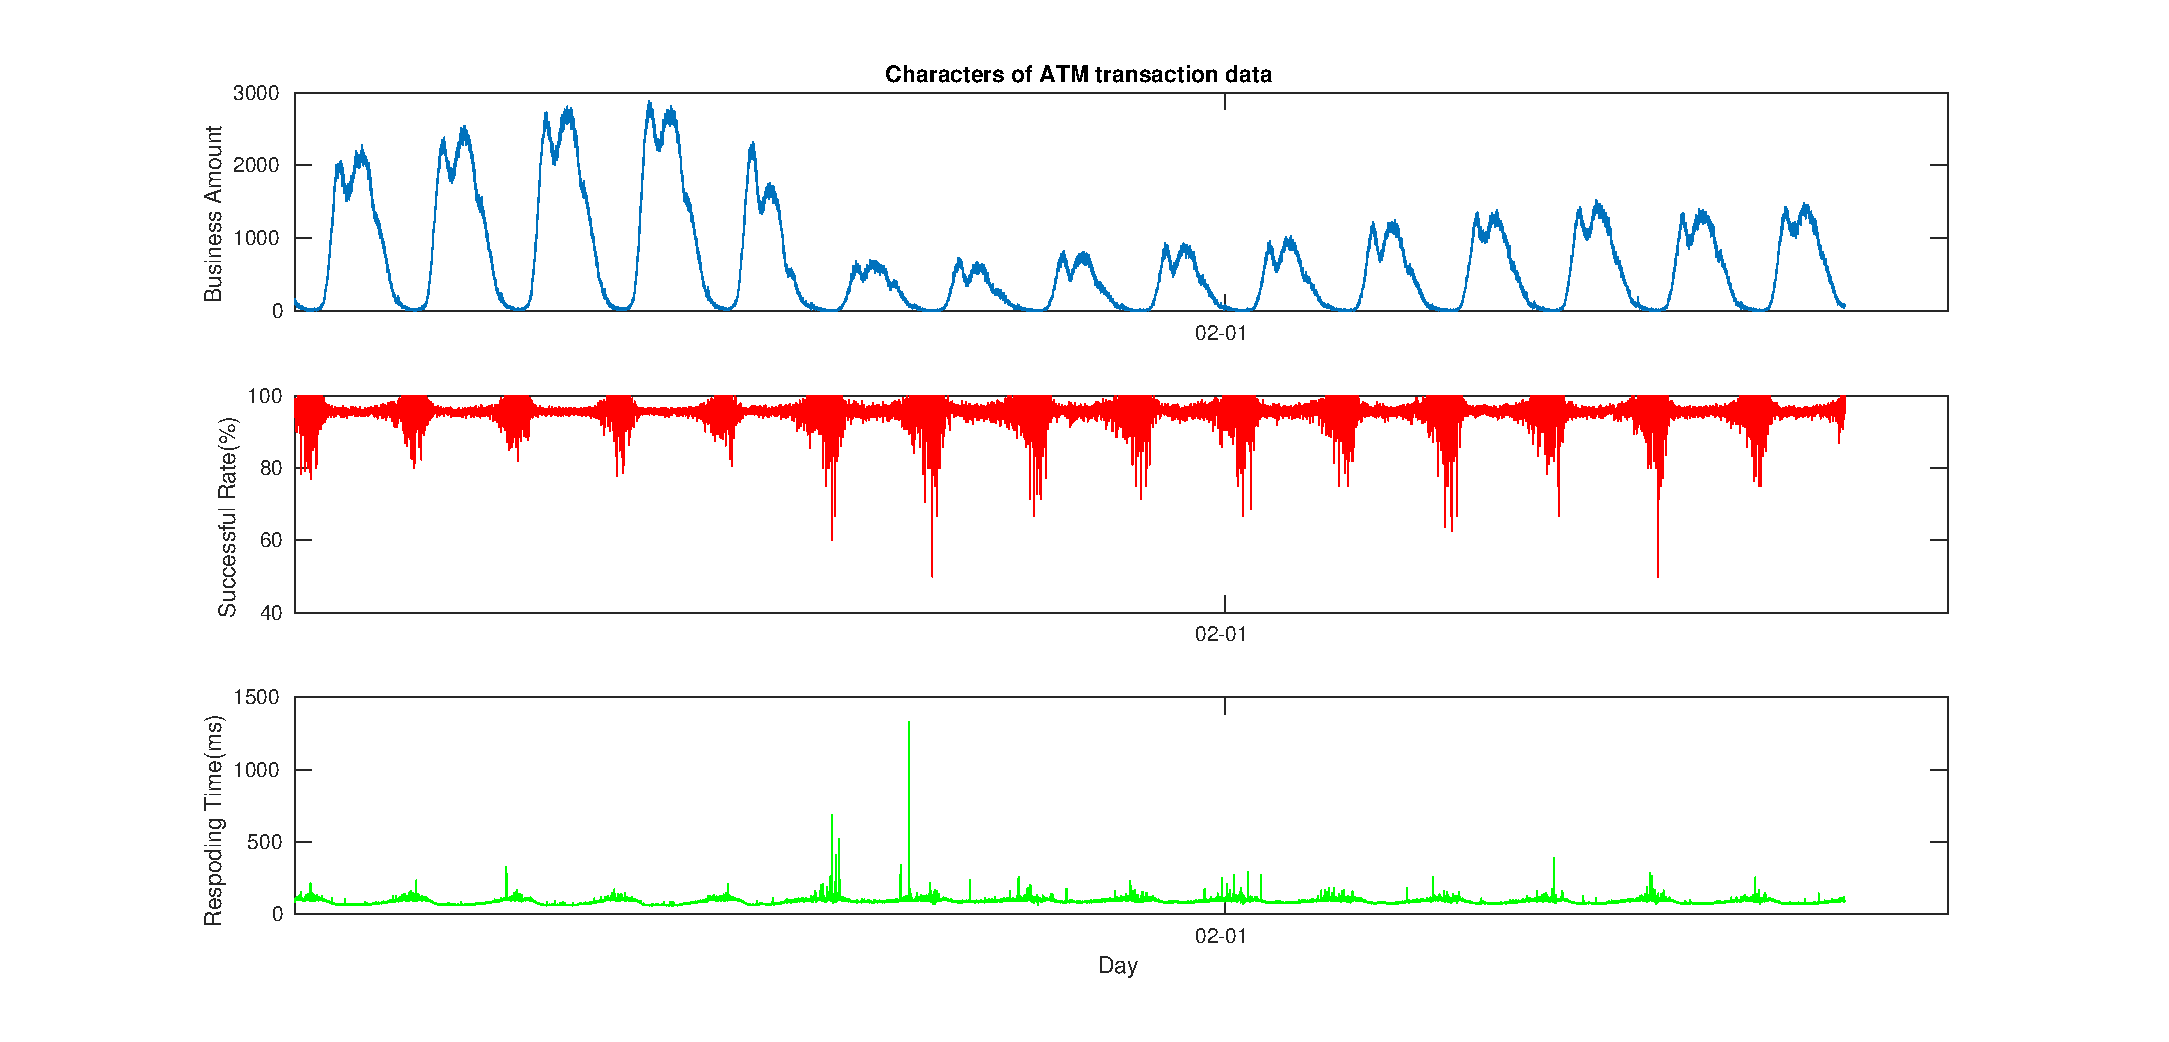
\includegraphics[scale=0.4]{pic/jan-feb-bsr.eps}
	\caption{ATM交易状态变化}
     \label{fig:char}
\end{figure}
ATM 业务状态随着时间是不断变化的;这种变化不仅仅是发生在每一天之内,同时也是存在于相邻两天的差异中。
通过对图 \ref{fig:char} 的观察可知,业务状态呈现以天为单位的周期变化,每一天的曲线大致相似但是有所区别。
为了在最少的特征参量下尽可能准确地描述业务状态的变化,我们可以通过将每一天的数据按时间划分成不同的模式。
对于每一种模式,我们会采用不同的特征参量来描述,这些特征参量在每个时间段内具有一定的稳定性。
\\
\section*{记号表}
\begin{table}[H]
	\centering
	\caption{}
	\label{tab:problem1_symbols}
	\begin{tabular}{ccc}
		\hline
		符号 & 含义 & 备注 \\
		\hline
		$t$ & Time & \\
        $B(t)$ & 业务量 & $[t, t+1)$ 内的累计业务量 \\
		$S(t)$ & 成功率 & $[t, t+1)$ 内的平均成功率 \\
		$R(t)$ & 响应时间 & $[t, t+1)$ 内的平均响应时间 \\
		$M_T^i$ & 中位数 & $T \in \{B, S, R\}$ \\
        $\sigma_T^i$ & 标准差 & $i \in \{1, 2, 3, 4\}$ \\
		$\tilde{\sigma}_T^i$ & 带修正的标准差 & 剔除原数据中落在 $c \cdot \sigma_T^i$ 外之后重新计算得到 \\
		$\vartheta_B^i$ & 斜率 & \\
        $r_B^i$ & 相关系数 & 最小二乘法拟合第 2、4 个时间段的相关系数\\
		\hline
	\end{tabular} \\
\end{table}
通过对数据的分析,总的来说,$B(t)$,$S(t)$,$R(t)$ 对于时间 $t$ 大致呈周期分布,且在每一个周期内的不同时间段会显示出不同的模式。
为了描述这些模式,我们主要通过中位数 $M$ ,标准差 $\sigma_T^i$ (与带有修正的标准差 $\tilde{\sigma}_T^i$ ) ,斜率 $\vartheta_B^i$ 这些特征参量来表征不同的状态。
\\
值得注意的是,我们可以很明显地从图 \ref{fig:char} 中看出一月份的业务量数据波动是非常大的。
由于一月底春节的影响,银行的业务量呈现与平日不同的模式,对于参数的估计是不利的,因此\emph{下文进行参数计算时选择的是二月至四月的数据}。

\section{业务量的特征参数}
\indent 业务量是指总行接收到的支行业务总数。
对于业务量 $B(t)$ ,我们将一天划分成四个时段,即:6 $\sim$ 9点,9 $\sim$ 18点,18 $\sim$ 23点,以及23 $\sim$ 次日6点,可参见图 \ref{fig:char_feb-1}。
对于每一个时段,业务量都有一些鲜明的特征,数据参见表 \ref{tab:char_B} 。
\begin{table}[H]
	\centering
	\caption{业务量特征参数}
	\label{tab:char_B}
	\begin{tabular}{c|cc|c|c|cc|cc}
		\hline
		\multirow{2}{*}{时间段 $i$} & \multicolumn{2}{c}{$M_B^i$} & $\sigma_B^i$ & $\tilde{\sigma}_B^i$ & \multicolumn{2}{c}{$\vartheta_B^i$} & \multicolumn{2}{c}{$r_B^i$} \\
		& mean         & sd           & mean        & mean                 & mean             & sd               & mean         & sd           \\
		\hline
		6-9 1                    & 406.73       & 121.87       & 289.16      & 286.19               & 5.4751           & 0.80011          & 0.98275      & 0.011052     \\
        9-18 2                   & 1053.9       & 108.17       & 102.34      & 96.315               & -$^{(*)}$     & -                & -            & -            \\
		18-23 3                  & 558.95       & 95.123       & 274.21      & 273.8                & -3.134           & 0.50446          & -0.9896      & 0.002531     \\
		23-(6) 4                 & 27.744       & 3.8689       & 29.158      & 23.813               & -                & -                & -            & -           \\
		\hline
	\end{tabular}
\end{table}
(*) \emph{对于日间与夜间业务量稳定的模式,其斜率没有显著的含义,因此未计算斜率与相关系数。}
\begin{figure}[htbp]
	\centering
	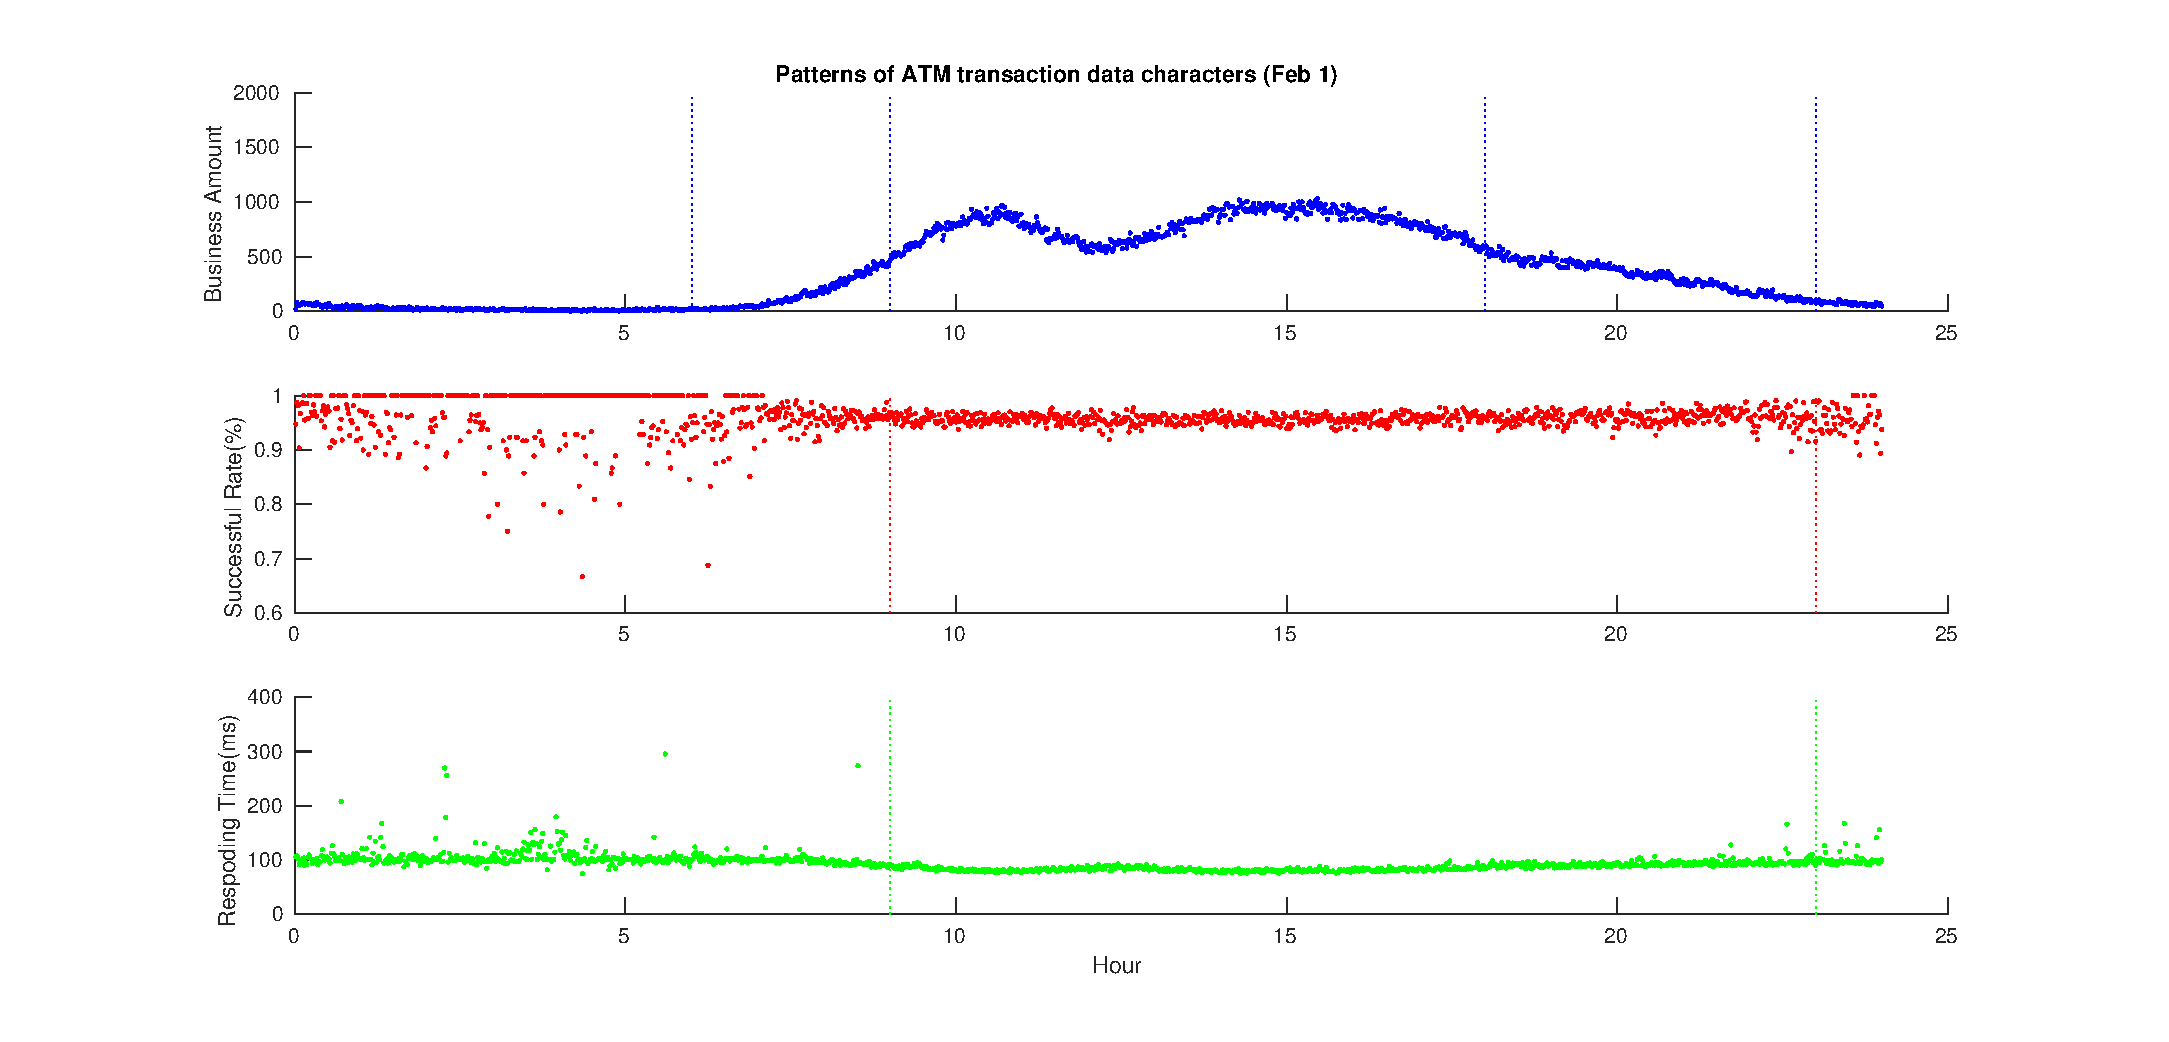
\includegraphics[scale=0.4]{pic/feb-1-bsr-pattern.eps}
	\caption{业务量、成功率、响应时间的典型分布}
    \label{fig:char_feb-1}
\end{figure}
\begin{itemize}
    \item 对于 6 $\sim$ 9 点,是业务量上升阶段,这个时段,平均值的意义不是很明显,这里我们用其上升的速度,也即斜率 $\vartheta_B^1$ 来表征这一时段的特点。
    \item 9 $\sim$ 18 点是一天中业务最为繁忙的一个时期。业务量大,同时波动的幅度也比较明显。所以,这段时间内中位数 $M_B^2$ 较大,标准差 $\sigma_B^2$ 也很大
    \item 第三个时间段是 18 $\sim$ 23 点,这段时间是业务下降阶段。与 6 $\sim$ 9 点类似,我们也用斜率 $\vartheta_B^3$来记录这一时期的特征。
    \item 对于 23 $\sim$ 次日 6 点,由于是夜间,客户往往不会选择在这段时间办理业务。所以业务量较少,波动不明显,从而 $M_B^4$ 和 $\sigma_B^4$ 都比较小。
\end{itemize}
进一步的,通过对比每一天的业务量的这些特征参量,我们发现每一天的趋势基本相同,即每一天这四个时段的趋势基本相同。
但具体到数值上时,有较大的偏差。
由表 \ref{tab:char_B} 的数据可以看出,日间的中位数的标准差要远大于每日标准差的平均值。
为了降低异常点对于特征参量数值的影响,将每日偏离中位数 $c$ 倍标准差外的数据予以剔除,并重新求标准差,得到表 \ref{tab:char_B} 第五列 $\tilde{\sigma}_B^i$ 的数据。
\\
\indent 对业务量异常点的出现原因,我们有以下分析:业务量是指总行接收到的支行业务总数。
当业务量陡然减少时,由于业务量数据是由支行节点通过网络传给总行,所以此时的故障很有可能为支行与总行的网络中断导致的。

\section{成功率的特征参数}
\indent 成功率的模式比较简单,主要分为两个时段,可参见图 \ref{fig:char_feb-1},数据参见表 \ref{tab:char_S} 。
\begin{table}[H]
	\centering
	\caption{成功率特征参数}
	\label{tab:char_S}
	\begin{tabular}{c|cc|c|c}
		\hline
		\multirow{2}{*}{时间段 $i$} & \multicolumn{2}{c}{$M_S^i$} & $\sigma_S^i$ & $\tilde{\sigma}_S^i$ \\
		& mean        & sd            & mean        & mean                 \\
		\hline
		9-23 1                   & 0.95683     & 0.00097769    & 0.0092547   & 0.0074817            \\
		23-(9) 2                 & 0.96463     & 0.0022323     & 0.0394      & 0.027581            \\
		\hline
	\end{tabular}
\end{table}
9 点至 23 点业务量繁多,银行后台的稳定性要求很高,所以这段时间的成功率的标准差比较小。
而 23 点至次日 9 点这段时间,由于这段时间业务量少,所以银行的通讯线路会非常通畅。
但另一方面,也由于业务较少,银行后台要求的稳定性有所降低;
考虑到银行的机器或者程序的检修一般都在晚上进行,不确定因素增加,所以这个时间段数据相对比较分散,标准差 $\sigma_S^2$ 很大,有时成功率能达到 100\% ,有时则会很低。
\\
\indent 影响交易的成功与否的因素很多,比如分行的数据变更或者配置错误、总行的数据中心后端处理系统应用进程异常等等。
若出现上述错误时,就会导致交易成功率下降。所以当成功率出现异常点时,应该及时检查是否这几个地方出现了问题。


\section{响应时间的特征参数}
\indent 响应时间的模式也主要分为两个时段,可参见图 \ref{fig:char_feb-1},数据参见表 \ref{tab:char_R} 。
\begin{table}[H]
	\centering
	\caption{响应时间特征参数}
	\label{tab:char_R}
	\begin{tabular}{c|cc|c|c}
		\hline
		\multirow{2}{*}{时间段 $i$} & \multicolumn{2}{c}{$M_S^i$} & $\sigma_S^i$ & $\tilde{\sigma}_S^i$ \\
		& mean        & sd            & mean        & mean                 \\
		\hline
		9-23 1                   & 83.212     & 9.0861    & 16.031   & 5.8181            \\
		23-(9) 2                 & 100.72     & 7.9057     & 194.53      & 17.266            \\
		\hline
	\end{tabular}
\end{table}
从 9 点至 23 点业务量巨大,银行必须使用大量的服务器才能满足客户业务量的需求,同时还要尽量减少响应时间以获得更多的业务量。
而对于 23 点至次日 9 点则相反,由于业务量较少,所以即使响应时间较慢也不会影响银行的处理效率;
同时出于降低能耗的原因,银行很有可能会减少夜间服务器的数量,从而使得这期间的响应时间 $R(t)$ 的中位数较大。
\\
\indent 响应时间主要受到总行数据中心后台处理系统的影响。
当处理系统异常,比如CPU负荷过大时,就会导致交易处理过程缓慢,进而导致响应时间过长。

\section*{小结}
通过上面的讨论,我们对这三项指标反应的 ATM 交易状态特性有了初步的了解,提取出了每个指标的特征参数,并对每个指标中出现奇异点的原因进行了分析。

\part{交易状态异常检测方案}
\section{引述}
\indent 通过分析数据,我们发现交易状态关于时间有明显的周期性趋势,但在不同的周期中,也有一些差异。要找出异常点,从来理论上来说,就是要找到一个对三个指标进行预测的模型,并将实际值与预测值相比较,当误差超过预先设定的阈值时,我们就认为出现了异常点。经过比较不同算法的优劣,我们最终采用了SSA算法作为我们的预测算法。  \\
\indent 对于我们研究的这三个指标,我们可以将它们看成是一串时间序列$F=(f(t_0),f(t_1),....,f(t_N-1))$,其中f表示B(t),S(t),R(t)。$N$为这一时间序列的长度。通过前面的分析,我们知道这串序列有一个弱周期T=1天。我们要做的就是通过目前的数据去预测短期的各项指标值。

\part{基于SSA算法的含噪声时间序列预测}
\section*{Symbols}
\begin{table}[H]
	\centering
	\caption{}
	\label{tab:ssa_symbols}
	\begin{tabular}{ccc}
		\hline
		符号 & 含义 & 备注 \\
		\hline
		$L$ & windows length & \\
		$N$ & the sample numbers & \\
		$f_i$ & the value of f at time i & $f \in \{B, S, R\}$ \\
		$\textbf{X}$ & trajectory matrix & \\
		$d$ & number of non-zero characters & \\
		$r$ & number of primary singular values & \\
		$a_i$ & coeffiencients of LRF & \\
		\hline
	\end{tabular} \\
\end{table}
\section{时间序列的分解}
\subsection{Trajectory}
\begin{equation}
	\label{eqn:F_i}
	F_i = (f_{i-1}, \cdots, f_{i+L-2})^T  (1 \leq i \leq K = N - L + 1)
\end{equation}

\begin{equation}
	\label{eqn:X}
	\textbf{X} = (F_1, \cdots, F_K)
\end{equation}

\subsection{SVD}

\begin{equation}
	\label{eqn:S}
	S = \textbf{X} \textbf{X}^T
\end{equation}

$S$ has characters $\lambda_i$ and according character vector $U_i$

\begin{equation}
	\label{eqn:V_i}
	V_i = \textbf{X}^T U_i / \sqrt{\lambda_i}
\end{equation}

\begin{equation}
	\label{eqn:X_i}
	\textbf{$X_i$} = \sqrt{\lambda_i} U_i V_i^T
\end{equation}

\begin{equation}
	\label{eqn:SVD_expanded}
	\textbf{X} = \Sigma_{i=1}^d \textbf{$X_i$}
\end{equation}
where
\begin{equation}
	\label{eqn:non-zero-char-d}
	d = max\{i \textbar \lambda_i > 0\}
\end{equation}
and we choose $r$ to be less than $d$.

\subsection{Reconstruction}
based on \ref{eqn:SVD_expanded} we can define
\begin{equation}
	\label{eqn:SVD}
	\textbf{X} = \textbf{U} \Sigma \textbf{V}^T
\end{equation}
where
\begin{equation}
	\label{eqn:SVD_U}
	\textbf{U} = (U_1, \cdots, U_K)
\end{equation}
\begin{equation}
	\label{eqn:SVD_Sigma}
	\Sigma = diag(\sqrt{\lambda_1}, \cdots, \sqrt{\lambda_K})
\end{equation}
\begin{equation}
	\label{eqn:SVD_V} 
	\textbf{V} = (V_1, \cdots, V_L)
\end{equation}

def of $a_i$
\begin{align}
	\textrm{R} &= (a_{L-1}, \cdots, a_1)^T \\
	           &= \frac{1}{1-\nu^2} \Sigma_{i=1}^r \pi_i U_i^\nabla \label{eqn:R_a}
\end{align}
where $\pi_i$ is the last component of the vector $U_i$, $U_i^\nabla$ is exactly $U_i$ but for the last component, and
\begin{equation}
	\label{eqn:ssa_nu^2}
	\nu^2 = \Sigma_{i=1}^r \pi_i^2
\end{equation}

\subsection{prediction}
as simple as
\begin{equation}
	\label{eqn:ssa_prediction}
	\tilde{f}_N = \Sigma_{i=1}^{L-1} a_i \cdot f_{N-L+i} 
\end{equation}

Add $\tilde{f}_N$ to $F$, we get
\begin{equation}
	\label{eqn:ssa_new_f}
	\tilde{F} = (f_0, \cdots, f_{N-1}, \tilde{f}_N)
\end{equation}
use $\tilde{F}$ to generate $\tilde{X}$, and finally iterate.

\section{异常检测模型}
我们作出如下假定
\begin{itemize}
    \item 对于某一时刻 $t$ ,量 $f(t)$ 的分布服从随 $t$ 变化的正态分布 $N(M(t), \sigma^2(t))$ 。
    \item 对于某一时刻 $t$ ,量 $f$ 出现异常,异常值 $\tilde{f}(t)$ 的分布服从随 t 变化的正态分布 $N(\tilde{M}(t), \tilde{\sigma}^2(t))$ 。
    \item 异常情况与正常情况的分布是独立的。
\end{itemize}

consider given t, M(t) -> M

the stocastic variable $\xi$ describes f , with $\mu$ decribing ~f

\begin{equation}
	\label{eqn:det_xi}
	\xi \sim N(M, \sigma^2)
\end{equation}

\begin{equation}
	\label{eqn:det_mu}
	\mu \sim N(\tilde{M}, \tilde{\sigma}^2)
\end{equation}

alarm level a

false alarm $p_f(a)$
\begin{align}
	p_f(a) &= P\{\xi < a\} \\
		&= \Psi(\frac{a-M}{\sigma}) \label{eqn:det-p_f}
\end{align}

hit $p_h(a)$
\begin{align}
	p_h(a) &= P\{\mu < a\} \\
		&= \Psi(\frac{a-\tilde{M}}{\tilde{\sigma}}) \label{eqn:det-p_h}
\end{align}

what is psi
\begin{equation}
	\label{eqn:psi}
	\Psi(x) = \int_{-\infty}^{x} \frac{1}{\sqrt{2\pi}}e^{-\frac{t^2}{2}} dt
\end{equation}

some pictures describing $p_f$ and $p_h$

want to select the best point (of course in terms of $a$) to raise sensitivity

several ways
\begin{enumerate}
	\item minizes $\sqrt{(p_h - 1)^2 + (p_f - 0)^2}$
	\item satisfies $p_f + p_h = 1$
	\item maximizes $p_h - p_f$
\end{enumerate} 

we use the simpliest way 
\begin{equation}
	\label{eqn:det_a_formula}
	\frac{a-M}{\sigma} = \frac{a-\tilde{M}}{\tilde{\sigma}}
\end{equation}
solve that
\begin{equation}
	a = \frac{\tilde{\sigma}M - \sigma \tilde{M}}{\tilde{\sigma} - \sigma}
\end{equation}

\section{与其他方法的比较分析}
\section{对方案可靠性的评估}
\section{不同突变点原因分析}

\part{方案的优化及完善}


\end{document}
